% Todo documento é iniciado pelo \documentclass
\documentclass[11pt,twocolumn]{article}

\usepackage[brazil]{babel}
\usepackage[utf8]{inputenc}
\usepackage[T1]{fontenc}

\usepackage{graphicx}
\usepackage[caption=false]{subfig}

% Definição das variáveis do texto
\title{Exemplo de Documento \LaTeX}
\author{Chauã Queirolo}
%\date{}

% Ambiente document: onde fica o conteúdo do texto
\begin{document}

% Criar o título do documento
\maketitle

\tableofcontents


% O documento é organizado em seções
% \part -> book
% \chapter{capitulo} -> book / report
% \section{seção}
% \subsection{subseção}
% \subsubsection{subsubseção}

\section{Introdução}
\label{sec_introducao}

Lorem ipsum dolor sit amet, consectetur adipiscing elit. Aenean facilisis est vitae dui pulvinar viverra. Orci varius natoque penatibus et magnis dis parturient montes, nascetur ridiculus mus. Suspendisse et dui tincidunt, rutrum leo vitae, feugiat odio. Cras hendrerit purus at venenatis dictum. Proin eros sem, bibendum sollicitudin interdum vitae, tempor sit amet felis. Duis pharetra rutrum eros fermentum hendrerit. Donec dignissim tincidunt euismod. Como visto na Seção~\ref{sec_introducao}.

Nam dictum mauris et diam convallis, sed sagittis dolor blandit. Fusce iaculis, mi eu molestie ullamcorper, lectus nibh scelerisque sem, nec pulvinar massa purus sit amet quam. Integer nec ante et purus lobortis feugiat ac ac velit. Duis pellentesque tincidunt ex, a pulvinar sem pharetra nec. Cras egestas velit vel consectetur dapibus. Vivamus in enim sed lacus egestas tempor. Phasellus bibendum sagittis rhoncus. Aliquam semper, turpis vitae vestibulum accumsan, ligula felis cursus quam, vitae suscipit ipsum velit sit amet ipsum. Nunc laoreet erat vel pretium venenatis. Nulla facilisi. Mauris tincidunt nisl vel massa placerat vulputate. Fusce porta est in velit commodo maximus. Sed ac tempor libero.

Exemplo de texto em \textbf{negrito}, \textit{itálico} e com \emph{ênfase}.

\section{Fundamentação Teórica}

\subsection{Algoritmo X}

Nam dictum mauris et diam convallis, sed sagittis dolor blandit. Fusce iaculis, mi eu molestie ullamcorper, lectus nibh scelerisque sem, nec pulvinar massa purus sit amet quam. Integer nec ante et purus lobortis feugiat ac ac velit. Duis pellentesque tincidunt ex, a pulvinar sem pharetra nec. Cras egestas velit vel consectetur dapibus. Vivamus in enim sed lacus egestas tempor. Phasellus bibendum sagittis rhoncus. Aliquam semper, turpis vitae vestibulum accumsan, ligula felis cursus quam, vitae suscipit ipsum velit sit amet ipsum. Nunc laoreet erat vel pretium venenatis. Nulla facilisi. Mauris tincidunt nisl vel massa placerat vulputate. Fusce porta est in velit commodo maximus. Sed ac tempor libero.

\subsection{Algoritmo Y}

Nam dictum mauris et diam convallis, sed sagittis dolor blandit. Fusce iaculis, mi eu molestie ullamcorper, lectus nibh scelerisque sem, nec pulvinar massa purus sit amet quam. Integer nec ante et purus lobortis feugiat ac ac velit. Duis pellentesque tincidunt ex, a pulvinar sem pharetra nec. \\
Cras egestas velit vel consectetur dapibus. Vivamus in enim sed lacus egestas tempor. Phasellus bibendum sagittis rhoncus. Aliquam semper, turpis vitae vestibulum accumsan, ligula felis cursus quam, vitae suscipit ipsum velit sit amet ipsum. Nunc laoreet erat vel pretium venenatis. \\
Nulla facilisi. Mauris tincidunt nisl vel massa placerat vulputate. Fusce~porta est in velit commodo maximus. Sed ac tempor libero.

\section{Exemplo com tabelas}

No \textit{tabular} são passados os parâmetros da tabela. A Tabela~\ref{tabela_exemplo} apresenta um exemplo de tabela.

\begin{table}[h]
  \centering
  \caption{Legenda da tabela.}
  \label{tabela_exemplo}
  \begin{tabular}{ |l||c|r| }
    \hline
    Primeira  & Segunda  & Terceira  \\ \hline\hline
    A & B & C \\ \hline
    A & B & C \\ \hline
    A & B & C \\ \hline
  \end{tabular}
  
\end{table}

\section{Exemplo com figuras}

A Figura~\ref{fig_exemplo} apresenta um exemplo de figura.

\begin{figure}[h]
\centering
  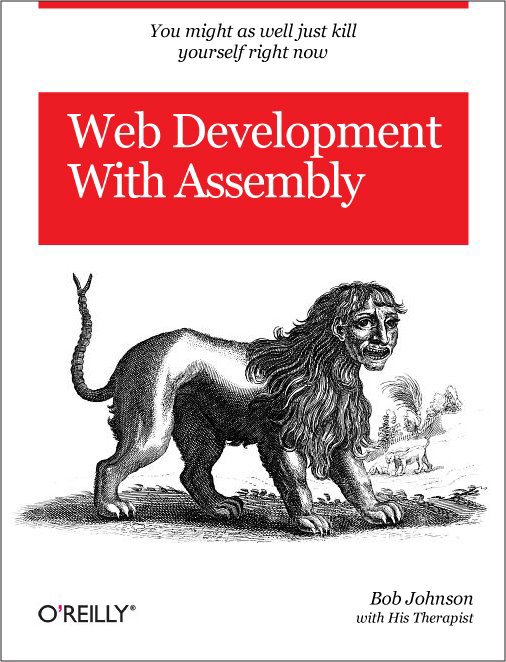
\includegraphics[width=6cm]{exemplo.jpg}
  \caption{Exemplo de figura.}  
  \label{fig_exemplo}
\end{figure}

\begin{figure}[h]
\centering
  \subfloat[][Exemplo 1]{
    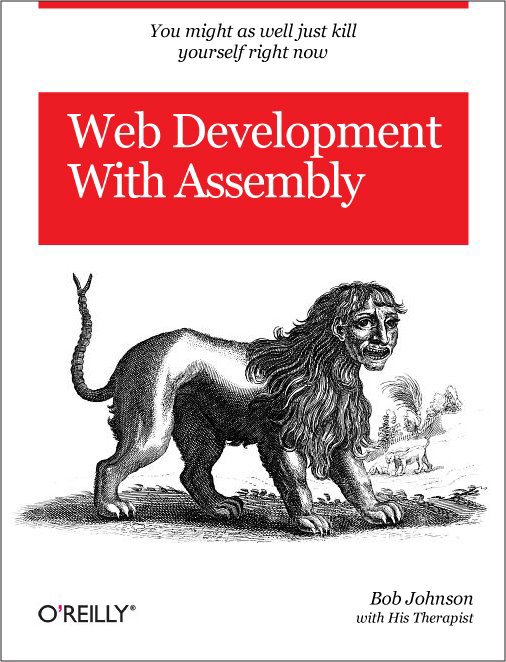
\includegraphics[width=3cm]{exemplo.jpg}
  }
  \subfloat[][Exemplo 2]{
    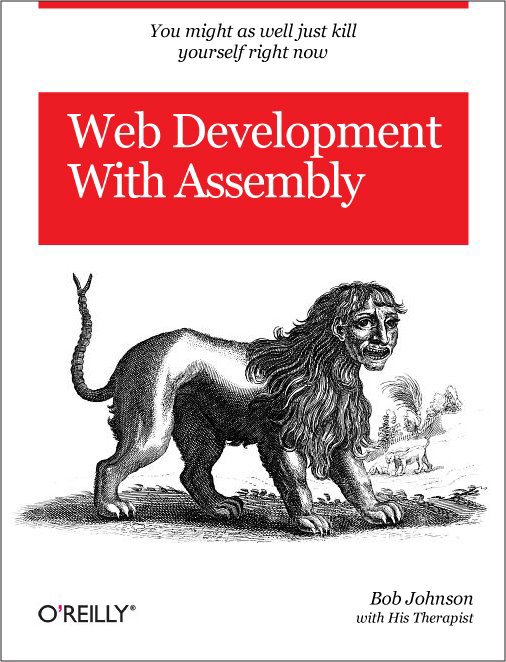
\includegraphics[width=3cm]{exemplo.jpg}
  }
  
  \subfloat[][Exemplo 1]{
    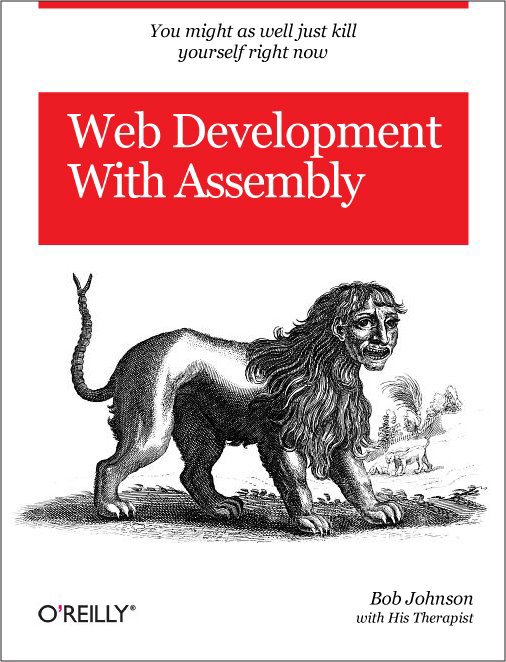
\includegraphics[width=3cm]{exemplo.jpg}
  }
  \subfloat[][Exemplo 2]{
    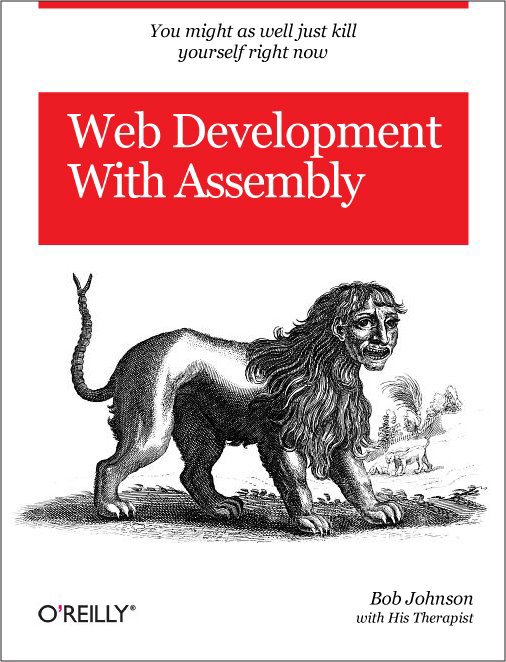
\includegraphics[width=3cm]{exemplo.jpg}
  }
  
  \caption{Exemplo de figura.}  
  \label{fig_exemplo}
\end{figure}


\section{Exemplo de listas}

A lista de itens de compra são: 

\begin{itemize}
  \item Café
  \item Açúcar
  \item Farinha
  \item Bolo
\end{itemize}

A lista de itens de compra são: 

\begin{enumerate}
  \item Café
  \item Açúcar
  \item Farinha
  \item Bolo
\end{enumerate}

A lista de itens de compra são: 

\begin{description}
  \item [Café] Pra poder tomar
  \item [Açúcar] Pra fazer o bolo
  \item [Farinha] Pra fazer o bolo
\end{description}

\section{Fórmulas}

Seja $x$ uma variável inteira e $y_1$ uma variável  real, então $\frac{x}{y_1}$ é a divisão. O valor do $\delta$ é o maior dos valores.

$$
x = \sqrt{y_1 + y_2}
$$

Conforme apresentado na Equação~\ref{eq_soma}.

\begin{equation}
\label{eq_soma}
A = \frac{\pi r^2}{2} = \frac{1}{2} \pi r^2 
\end{equation}







\end{document}
